\documentclass{article}
\usepackage{times}
\usepackage{graphicx}
\usepackage{subfigure} 
\usepackage{natbib}
\usepackage{algorithm}
%\usepackage{algorithmic}
\usepackage{algpseudocode}
\usepackage{amsmath}
\usepackage{hyperref}
\newcommand{\theHalgorithm}{\arabic{algorithm}}
\usepackage{icml2015stylefiles/icml2015} 
%\usepackage[accepted]{icml2015stylefiles/icml2015}


\newcommand{\vx}{\mathbf{x}}
\newcommand{\vv}{\mathbf{v}}
\newcommand{\vg}{\mathbf{g}}
\newcommand{\vzero}{\mathbf{0}}
\newcommand{\ones}[1]{\mat{1}_{#1}}
\newcommand{\eye}[1]{\mat{E}_{#1}}
\newcommand{\tra}{^{\mathsf{T}}}
\newcommand{\vect}[1]{{\bf{#1}}}
\newcommand{\mat}[1]{\mathbf{#1}}
\newcommand{\pderiv}[2]{\frac{\partial #1}{\partial #2}}
\newcommand{\npderiv}[2]{\nicefrac{\partial #1}{\partial #2}}

\newcommand{\numhypers}{N}
\newcommand{\hypers}{{\boldsymbol{\theta}}}
\newcommand{\params}{\vx}
\newcommand{\numsteps}{T}
\newcommand{\decay}{\gamma}
\newcommand{\decays}{{\boldsymbol{\decay}}}
\newcommand{\stepsize}{\alpha}
\newcommand{\stepsizes}{{\boldsymbol{\stepsize}}}
\newcommand{\gradparams}{\nabla_\params L(\params_t, \hypers, t)}

\newcommand\ourtitle{Gradient-based Hyperparameter Optimization through Reversible Learning}
\icmltitlerunning{\ourtitle} % A short form for the running title.

\begin{document} 

\twocolumn[
\icmltitle{\ourtitle}

% It is OKAY to include author information, even for blind
% submissions: the style file will automatically remove it for you
% unless you've provided the [accepted] option to the icml2015
% package.
\icmlauthor{Dougal Maclaurin}{maclaurin@physics.harvard.edu}
%\icmladdress{Harvard University, Cambridge, Massachusetts}
\icmlauthor{David Duvenaud}{dduvenaud@seas.harvard.edu}
%\icmladdress{Harvard University, Cambridge, Massachusetts}
\icmlauthor{Ryan P. Adams}{rpa@seas.harvard.edu}
%\icmladdress{Harvard University, Cambridge, Massachusetts}

% You may provide any keywords that you 
% find helpful for describing your paper; these are used to populate 
% the "keywords" metadata in the PDF but will not be shown in the document
\icmlkeywords{hyperparameters, neural networks, reversible computation, automatic differentiation, machine learning, ICML}

\vskip 0.3in
]

\begin{abstract} 
Tuning hyper-parameters of learning algorithms is hard because gradients are usually unavailable.
We compute exact gradients of cross-validation performance with respect to all hyperparameters by chaining derivatives through the \emph{entire training procedure}.
These gradients allow us to optimize thousands of hyperparameters, including step-size and momentum schedules, weight initialization distributions, richly parameterized regularization schemes, and neural network architectures.
We compute hyperparamater gradients efficiently by exactly reversing the dynamics of stochastic gradient descent with momentum.%, storing only the information lost due to finite precision arithmetic.
\end{abstract} 

\section{Introduction}
\label{intro}



\paragraph{Meta-optimization}

The current state-of-the-art for hyperparameter optimization is achieved by model-based, gradient-free methods~\cite{snoek2012practical, bergstra2011algorithms, BerYamCox13, HutHooLey11}.
These methods are able to effectively exploit the information learned through evaluations of the objective.
However, in general they are not able to effectively optimize more than 10 to 20 parameters.
Most importantly from our perspective, current hyper parameter optimization schemes do not usually have access to gradients with respect to these hyperparameters, although they could incorporate this information if it were available~\cite{solak2003derivative}.

\begin{figure}[ht]
\vskip 0.2in
\begin{center}
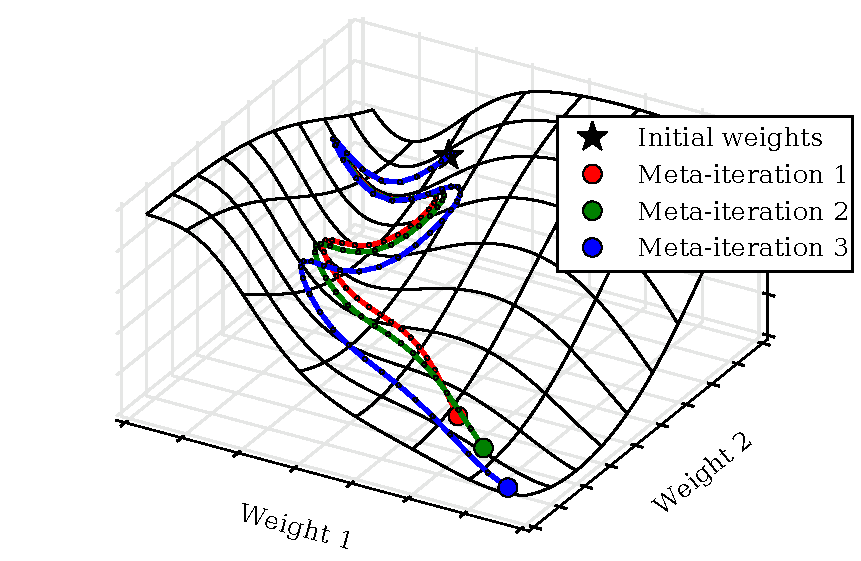
\includegraphics[width=\columnwidth]{../experiments/Jan_25_Figure_1/2/learning_curves.pdf}
\caption{Meta-optimization by gradient descent.
Each meta-iteration uses stochastic gradient descent to optimize parameters with respect to training error, holding hyperparameters fixed.
We then compute the gradient of the validation loss with respect to all hyperparameters.
These ``hyper-gradients'' are used to update the hyperparameters.}
\label{fig:chaos}
\end{center}
\vskip -0.2in
\end{figure}


\subsection{Contributions}

\begin{itemize}
\item We give an algorithm that exactly reversing stochastic gradient descent with momentum to compute gradients with respect to all continuous training parameters.
\item We show how to efficiently store only the information needed to exactly reverse learning dynamics.
For example, when the momentum term is 0.9, this method reduces the memory requirements of reverse-mode differentiation by factor of 200.
\item We show how these gradients allow the optimization of validation loss with respect to thousands of hyperparameters.
For example, we optimize fine-grained learning-rate schedules, per-layer initialization distributions, per-input regularization schemes, and even per-pixel data preprocessing.
\item We provide insight into learning procedures by examining optimized learning-rate schedules and initialization procedures, comparing them to standard advice in the literature.
\end{itemize}



\section{Automatic differentiation}

Automatic differentiation (AD) software packages such as Theano~\cite{Bastien-Theano-2012, bergstra2010scipy} are a workhorse of deep learning, significantly speeding up development time by providing gradients automatically.
However, these methods are typically only used to train parameters with respect to some loss.
\citet{Autodiff14} suggest using automatic differentiation to compute gradients with respect to hyperparameters.
However, naively applying automatic differentiation through hundreds of iterations of most learning procedures would either be prohibitively slow, or take prohibitive amounts of memory.

\subsection{Forward vs. Reverse-Mode Differentiation}
By the chain rule, the gradient of a set of nested functions is given by the product of the individual derivatives of each function:
%
\begin{align*}
\pderiv{f_4(f_3(f_2(f_1(x))))}{x} = \pderiv{f_4}{f_3} \cdot \pderiv{f_3}{f_2} \cdot \pderiv{f_2}{f_1} \cdot \pderiv{f_1}{x}
\end{align*}
If each function has multivariate inputs and outputs, the gradients can be replaced with Jacobian matrices.
%
Forward-mode AD works by multiplying gradients in the same order as the functions are evaluated:
%
\begin{align*}
\pderiv{f_4(f_3(f_2(f_1(x))))}{x} = \pderiv{f_4}{f_3} \cdot \left( \pderiv{f_3}{f_2} \cdot \left( \pderiv{f_2}{f_1} \cdot \pderiv{f_1}{x} \right) \right)
\end{align*}
%
In forward-mode, gradients can be computed at the same time as the original function, keeping track of the directional gradient.
This method has only twice the memory cost of simply computing the function of interest, but in general requires a separate forward pass for each input parameter, resulting in an $\mathcal{O}(\numhypers)$ slowdown, where $\numhypers$ is the number of input parameters.~\cite{pearlmutter2008reverse}

Reverse-mode AD works by maintaining a tape of computations performed, and computing the gradient in a backwards pass, starting from the final result:
%
\begin{align*}
\pderiv{f_4(f_3(f_2(f_1(x))))}{x} = \left(  \left(  \pderiv{f_4}{f_3} \cdot \pderiv{f_3}{f_2} \right) \cdot \pderiv{f_2}{f_1} \right) \cdot \pderiv{f_1}{x} 
\end{align*}
%
Naive reverse-mode AD typically only requires approximately twice the time as computing the original function, but can require up to $\mathcal{O}(\numsteps\numhypers)$ memory, where $\numsteps$ is the number of nested functions.
In sections \ref{sec:reversible learning} and \ref{sec:reversible computation}, we show how to drastically reduce the memory requirements of reverse-mode AD for differentiating through the entire learning procedure.

\section{Reversible learning}
\label{sec:reversible learning}

In the case of large neural networks, the amount of memory required to store the millions of parameters being trained is typically close to the amount of physical RAM available~\cite{sequence2014}.
Thus storing every intermediate parameter value throughout training in order to perform reverse-mode differentiation is completely impractical.
If storing the parameter vector takes $\sim$1GB, and the parameter vector is updated tens of thousands of times (equal to the number of mini batches times the number of epochs) then storing the learning history becomes unmanageable even with physical storage.

This section discusses how we overcome the technical difficulty of recovering the history of parameter vectors in order to perform reverse-mode AD, when performing stochastic gradient descent with momentum.

Stochastic gradient descent (SGD) with momentum (Algorithm \ref{alg:sgd}) can be seen as a physical simulation of a system moving through a series of fixed force fields indexed by time $t$.

%
\begin{algorithm}
   \caption{Stochastic gradient descent with momentum}
   \label{alg:sgd}
\begin{algorithmic}[1]
   \State {\bfseries input:} initial $\vx_1$, decays $\decays$, stepsizes $\stepsizes$, loss $L(\params, \hypers, t)$
   \State initialize $\vv_1 = \vzero$
   \For{$t=1$ {\bfseries to} $T$}
   \State $g_t = \gradparams$ \Comment{evaluate gradient}
   \State $\vv_{t+1} = \decay_t \vv_t - (1 - \decay_t) \vg_t$ \Comment{update velocity}  \label{step:update velocity}
   \State $\vx_{t+1} = \vx_t + \stepsize_t \vv_t$ \Comment{update position} \label{step:update position}
   \EndFor
   \State \textbf{output} trained parameters $\vx_T$
\end{algorithmic}
\end{algorithm}
%

We can view SGD as a function which takes an initial parameter vector, a step-size schedule, and a momentum schedule, and returns the final parameter vector.

The validation and test set performance depend on the output of this function, the trained weights.
It is usually straightforward to compute the gradient of the validation loss with respect to the trained weights.
To get hyper parameter gradients, we also need to differentiate the output of stochastic gradient descent with respect to its inputs.
How can we take the gradient of SGD with respect to its parameters?

\subsection{Reversible dynamics}

If the momentum decay term $\decay$ in Algorithm \ref{alg:sgd} is set to one, then we recover a reversible dynamics scheme known as the leapfrog integrator~\citep{leapfrog1995}.
%Leapfrog dynamics are exactly reversible through time.
Exactly reversible dynamics would allow us to trace a training procedure backwards, starting from the trained parameter values.
Having the parameter vectors available in this order would allow reverse-mode AD with fixed memory requirements, no matter how many training iterations were performed.

This procedure is given by Algorithm \ref{alg:reverse-sgd}, which simply reverses the steps in Algorithm \ref{alg:sgd}, interleaved with computations of gradients.
It outputs the gradient of a function of the trained weights $f(\vx)$ (such as the validation loss) with respect to the initial weights $\vx_1$, the stepsize and momentum schedules, and any other hyperparameters which affect training gradients.
%
\begin{algorithm}
   \caption{Reverse-mode differentiation of SGD \\ without checkpointing}
   \label{alg:reverse-sgd}
\begin{algorithmic}[1]
   \State {\bfseries input:} $\vx_T$, $\vv_T$, $\decays$, $\stepsizes$, train loss $L(\params, \hypers, t)$, loss $f(\params)$
   \State initialize $d\vv = \vzero$, $d\hypers = \vzero$, $d\stepsize_t = \vzero$, $d\decay = \vzero$
   \State initialize $d\vx = \nabla_\params f(\params_T)$
   \For{$t=T$ {\bfseries counting down to} $1$}
   \State $d\stepsize_t = d\vv\tra \vv_t$
   \State $\vx_{t-1} = \vx_t - \stepsize_t \vv_t$ \label{step:reverse-position}
   \vspace{-0.95\baselineskip}
   \State $\vg_t = \gradparams$ \label{step:reverse-gradient}
   \hfill \scalebox{1.1}{\Bigg\}} \vspace{-\baselineskip} \begin{minipage}{2.5cm} exactly reverse \\ gradient descent \\ operations \strut \end{minipage}
   \State $\vv_{t-1} = [\vv_t - (1 - \decay_t) \vg_t] / \decay_t$ \label{step:reverse-velocity}
   \State $d\vv = d\vv + \stepsize_t d\vx$
   \State $d\decay_t = d\vx\tra (\vv_t + \vg_t)$
   \State $d\vx = d\vx - (1 - \decay_t) d\vv \nabla_\params \gradparams$ \label{line:hvp1}
   \State $d\hypers = d\hypers - (1 - \decay_t) d\vv \nabla_\hypers \gradparams$ \label{line:hvp2}
   \State $d\vv = \decay_t d\vv$
   \EndFor
   \State \textbf{output} gradient of $f(\vx_T)$ w.r.t $\vx_1$, $\vv_1$, $\decays$, $\stepsizes$ and $\hypers$
\end{algorithmic}
\end{algorithm}
%

\paragraph{Time complexity}
Computations of steps \ref{line:hvp1} and \ref{line:hvp2} both require a Hessian-vector product, but these can be computed exactly in about the same time required to compute a gradient \citep{pearlmutter1994fast}.
%These gradients are in principle derivable by hand, but in order for this procedure to work without extra work by the user, we would require an automatic differentiation package which could compute second derivatives.
Thus the time complexity of reverse SGD is $\mathcal{O}(T)$, the same as forward SGD.

\subsection{Self-closed Automatic Differentiation}
\citet{pearlmutter2008reverse} implemented the first example of an automatic differentiation package that was closed under its own operation, meaning it could be used to take 2nd or 3rd gradients by simply applying the gradient operation more than once.
However, this package could only operate on code written in a limited form of Scheme in which each function could only have one argument.
Popular AD popular packages such as Theano do not have this ability to automatically compute higher-order gradients.
Thus, we implemented our own automatic differentiation package (available at \url{www.redacted.com}) for Python that is closed under its own operation.
This package has the additional feature that it operates on standard Numpy~\cite{oliphant2007python} code.

\subsection{The decay term causes non-reversibility}
%In practice, however, best performance is usually achieved when the decay term set to a value such as $0.98$.
%Even if the decay were less than one, if one could somehow simulate having exact real numbers, this procedure could be reversed, and used for reverse-mode AD.
The decay term must be less than one in order for the optimizer to converge.
Since information is lost each time decay is applied, and the learning process is no longer exactly reversible.
Even if double-precision floating point numbers are used, errors accumulate exponentially, and the reversed learning procedure ends far from the initial point.
This means that naively applying Algorithm \ref{alg:reverse-sgd} will not provide accurate gradients if the decay term is less than one.

\section{Reversible computation even with non-reversible dynamics}
\label{sec:reversible computation}
To get around the problem of information loss caused by decay, we need to store the information lost in each iteration.
One approach, known as checkpointing, simply stores the entire weight vector every few iterations. [Cite James Martens and RNNs]
However, this would require too much memory to be practical for large neural nets trained for thousands of minibatches.
Luckily, when the decay factor is close to 1, the amount of information lost at each iteration is small.

\textbf{Quantifying the Savings}
for example, an integer multiplied by 0.98 will lose $0.029$ bits of information on average.
Compared to storing a new 32-bit integer or floating-point number, 
Thus, if we needed only to store the small amount of information lost at each iteration, memory requirements would only be ${\frac{0.029}{32} = 0.1\%}$ of what they would otherwise be.
Even if the decay term is $0.5$, memory requirements are still only $\frac{1}{32}$ of what they would otherwise be.

\subsection{Storing Fractional Bits on a Tape}

for each parameter being updated during learning, we keep a tape of bits.
Each time an information-destroying operation (such as division by an integer) is performed, we store the information that would be needed to reverse the operation exactly.  In the case of division by an integer, this information is simply the remainder.
During the reverse pass, when the inverse operation is performed (multiplication by that same integer), this extra information is extracted from the tape.

Addition and subtraction are exactly reversible operations on fixed-precision numbers, except when overflow occurs.
%Thus step \ref{step:update position} in Algorithm \ref{alg:sgd} is exactly reversible with fixed-point arithmetic.
However, division or multiplication by a value less than one, in a fixed-point number system, causes information to be lost.
Thus in SGD when the current velocity is multiplied by a decay term less than 1 (step \ref{step:update velocity} in Algorithm \ref{alg:sgd}), information is lost about the initial trajectory of the learning process.
When this same step is revisited in the reverse-SGD algorithm (step \ref{step:reverse-velocity} in Algorithm \ref{alg:reverse-sgd}), this information must be added back into the result if the computation is to proceed backward along the same path.

Algorithm \ref{alg:reversible-mult} shows how to multiply an integer by a ratio in such a way that the information lost is stored in another integer $i$.
This integer acts as an ``information buffer'', which stores the extra information lost during the training process.
This same information is retrieved in reverse order in steps \ref{step:reverse-position}, \ref{step:reverse-gradient}, and \ref{step:reverse-velocity} of Algorithm \ref{alg:reverse-sgd}.

%
\begin{algorithm}
   \caption{Exactly reversible multiplication by a ratio}
   \label{alg:reversible-mult}
\begin{algorithmic}[1]
   \State {\bfseries Input:} Information buffer $i$, value $c$, ratio $n / d$
   \State $i = i \times d$ \Comment{make room for new digit}               \label{step:f1}
   \State $i = i + (c \! \mod d)$ \Comment{store digit lost by division}   \label{step:f2}
   \State $c = c \div d$ \Comment{divide by denominator}                   \label{step:f3}
   \State $c = c \times n$ \Comment{multiply by numerator}                 \label{step:b1}
   \State $c = c +  (i \! \mod n)$ \Comment{add digit from buffer}         \label{step:b2}
   \State $i = i \div n$ \Comment{shorten information buffer}              \label{step:b3}
   \State \textbf{return} updated buffer $i$, updated value $c$
\end{algorithmic}
\end{algorithm}
%

%Notice that steps \ref{step:f1}, \ref{step:f2}, and \ref{step:f3} are the same as steps \ref{step:b1}, \ref{step:b2}, and \ref{step:b3}, but with the two variables switched.
%
%\paragraph{How to store less than one bit?}
%In the case where $\decay$ is close to one, typically less than a single bit will be s
%
Algorithm \ref{alg:reversible-mult} is analogous to using arithmetic coding to store a random digit having a uniform distribution~\citep{steinruecken2014a}.

\section{Experiments}

In typical machine learning applications, only a few hyperparameters (less than 20) are optimized.
Since each experiment only yields a single number, the search rapidly becomes more difficult as the dimension of the hyper parameter vector increases.
%For a neural network, these usually include a global weight initialization scale, learning rate and momentum, along with various architecture choices [cite Dalh QSAR paper].
In contrast, when hyper-gradients are available, the amount of information gained from each training run grows along with the number of hyperparameters, allowing us to optimize thousands of hyperparameters.%allow us to optimize any continuous parameter upon which training depends.
How can we take advantage of this new ability?

This section shows some proof-of-concept experiments of ways in which we can more richly parameterize our training and regularization schemes that would have been previously impractical to optimize.

\subsection{Gradient-based optimization of gradient-based optimization}

Modern neural net training procedures often employ various heuristics to set learning rate schedules, or set their shape using one or two hyperparameters set by cross-validation \citep{dahl2014multi}, \citep{sutskever2013importance}

Having access to gradients allows us to optimize thousands of hyperparameters.

Each primal iteration uses a different set of random initial weights, as well as a random reshuffling of dataset.
This prevents the learning schedules from depending on quirks of the initial random initialization.

We refined Algorithms \ref{alg:sgd} and \ref{alg:reverse-sgd} to allow a separate step-size and momentum schedule for each type of parameter in each layer of layer.
%
\begin{figure}[h!]
\vskip 0.2in
\begin{center}
Optimized training schedule \\
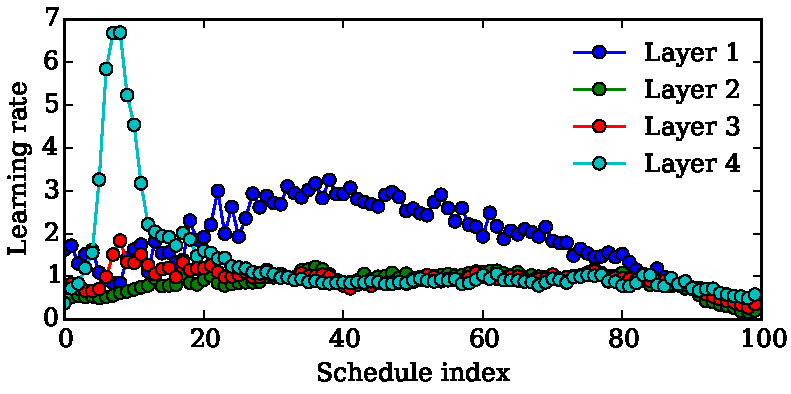
\includegraphics[width=\columnwidth]{../experiments/Feb_3_training_schedules/3_adam_50/schedules_small.pdf}
\caption{A step-size training schedule optimized by hyper-gradient descent.
The optimized schedule starts by taking large steps only in the topmost layer, then takes larger steps in the first layer.}
\label{fig:optimal schedule}
\end{center}
\vskip -0.2in
\end{figure} 
%
Figure {fig:optimal schedule} shows the results of optimizing learning rate schedules separately for each layer of a deep neural network.
The network had 4 layers, of size $[784, 50, 50, 50]$.

\begin{figure}[h!]
\vskip 0.2in
\begin{center}
Initial hyper-gradient\\
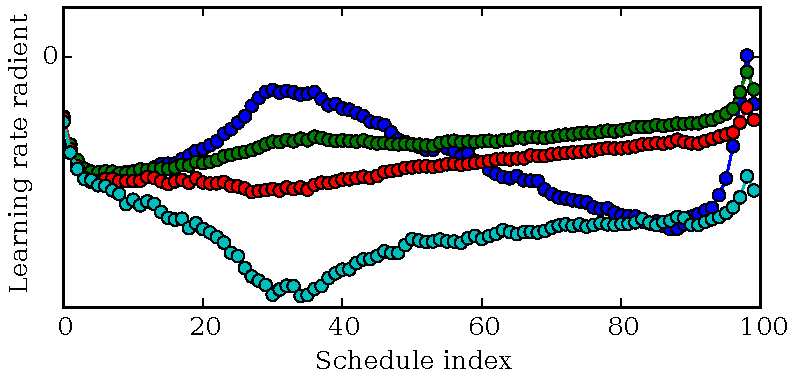
\includegraphics[width=\columnwidth]{../experiments/Feb_3_training_schedules/5_initial_gradient/schedules_small.pdf}
\caption{The initial gradient of the cross-validation loss with respect to the training schedule, averaged over 100 random weight initializations and mini batches.}
\label{fig:optimal schedule}
\end{center}
\vskip -0.2in
\end{figure} 

\paragraph{Weight initialization scales}
We also optimized the scale of random weight initialization separately for each layer, and separately for weights and biases in each layer.
Results are shown in figure \ref{fig:nn weight init scales}.

\begin{figure}[h!]
\vskip 0.2in
\begin{center}
\begin{tabular}{cc}
 Biases & Weights \\
\hspace{-1em}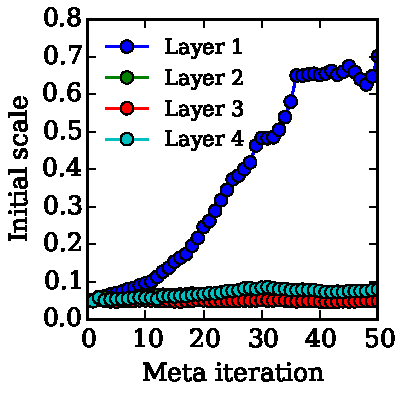
\includegraphics[width=0.5\columnwidth, height=0.5\columnwidth]{../experiments/Feb_3_training_schedules/3_adam_50/init_bias_learning_curve.pdf} &
\hspace{-1em}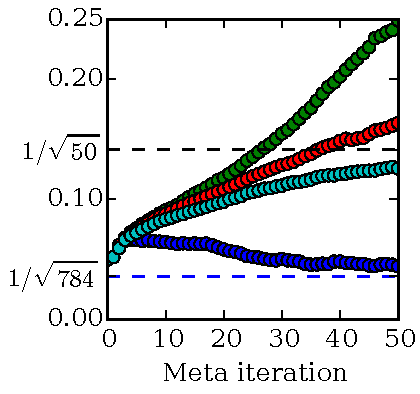
\includegraphics[width=0.5\columnwidth, height=0.5\columnwidth]{../experiments/Feb_3_training_schedules/3_adam_50/init_weight_learning_curve.pdf}
\end{tabular}
\caption{\emph{Top:} Meta-training curves for the initialization scales of different types of weights.
The meta-optimized weight distributions set the first layer weights to be small, and the second layer weights to be large.
Only one layer needs to be non-zero at initialization in order to break symmetry.}
\label{fig:nn weight init scales}
\end{center}
\vskip -0.2in
\end{figure} 

\subsection{Optimizing regularization parameters}

Regularization is often important for generalization performance is .
Typically, a single parameter controls a single L2 norm or sparsity penalty on the entire parameter vector of a neural network.
Because different types of parameters in different layers play different roles, it is reasonable to include a separate regularization hyperparameter for each parameter type.

\paragraph{Automatic relevance determination}
We can take this idea even further, and introduce a separate regularization penalty for each individual parameter in a neural network.
This

\begin{figure}[h!]
\begin{center}
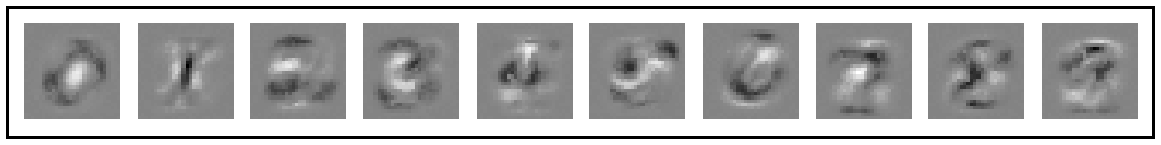
\includegraphics[width=\columnwidth]{../experiments/Jan_21_nn_ard/2/weights.pdf}
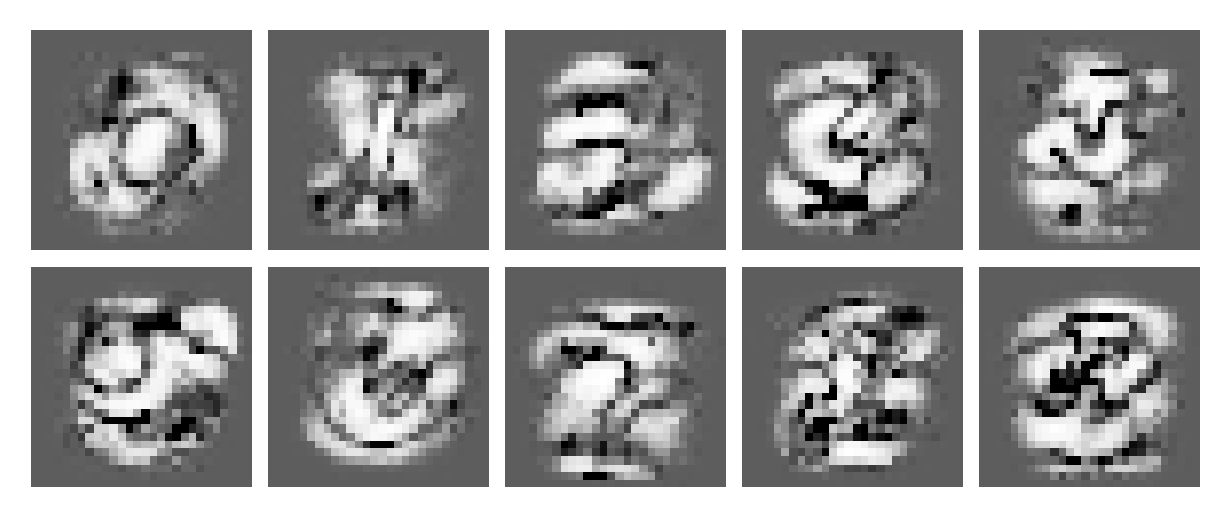
\includegraphics[width=\columnwidth]{../experiments/Jan_21_nn_ard/2/penalties.pdf}
\caption{\emph{Top:} Filters learned to classify MNIST in logistic regression.
\emph{Bottom:} L2 regularization hyperparameters for each weight..}
\label{fig:logistic ard}
\end{center}
\end{figure} 


\subsection{Optimizing data}

We can use Algorithm \ref{alg:reverse-sgd} to take the gradient with respect to any parameter the training procedure depends on.
This includes the training data, which can be viewed as just another set of hyper-parameters.
By chaining gradients through transformations of the data, we can compute gradients of the validation objective with respect to data preprocessing, weighting, or augmentation procedures.

We demonstrate a simple proof-of-concept where the \emph{entire training set} is learned by gradient descent.
%
\begin{figure}[h!]
\begin{center}
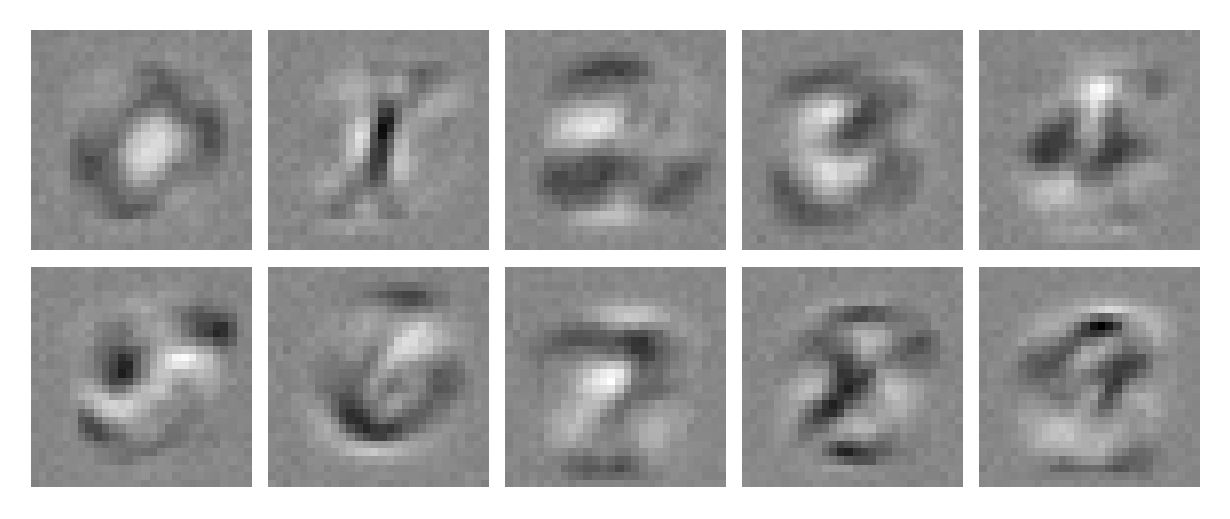
\includegraphics[width=\columnwidth]{../experiments/Jan_19_optimize_data/4/fake_data.pdf}
\caption{Fake data}
\label{fig:fake data}
\end{center}
\end{figure} 
%
Figure \ref{fig:fake data} shows a training set, the pixels of which were optimized to improve performance on a validation set of 10,000 examples from MNIST.


\subsection{Learning to Learn Languages}

\begin{figure}[h!]
\begin{center}
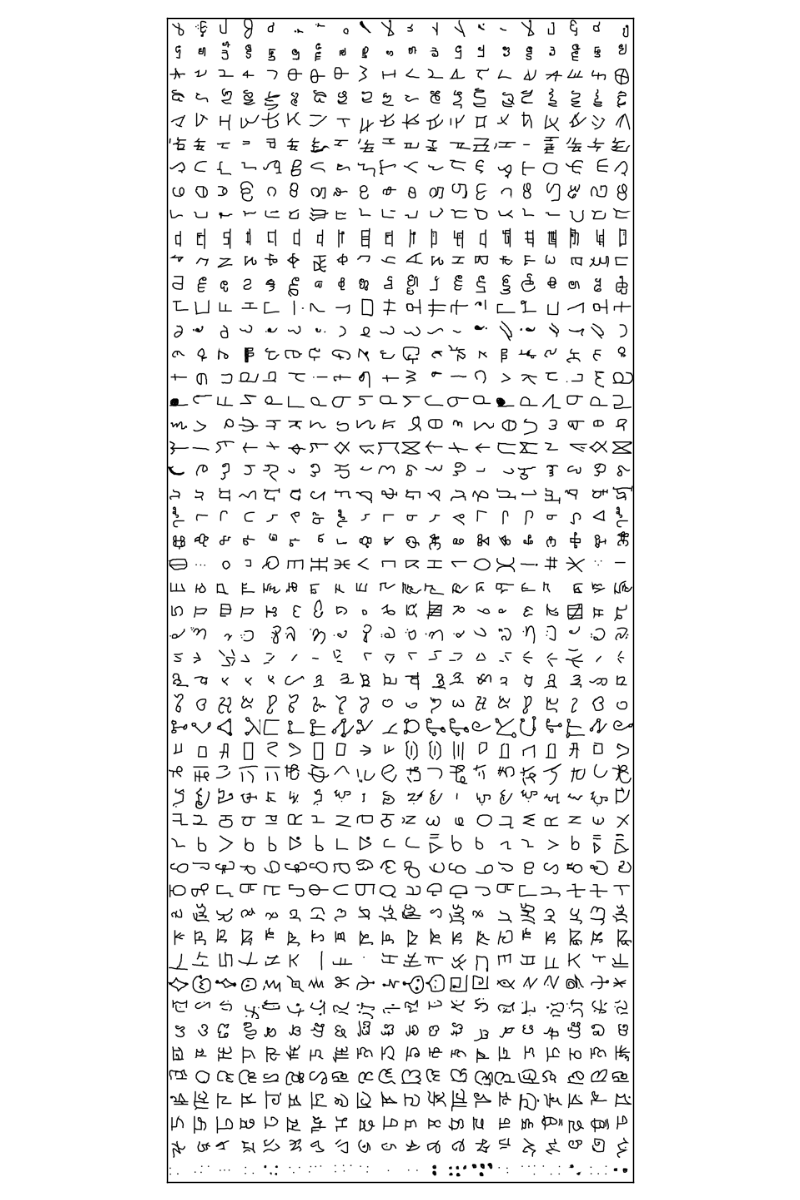
\includegraphics[width=\columnwidth, clip, trim=5cm 23cm 5cm 1cm]{../experiments/Feb_1_learning_alphabet_corr/5/all_alphabets.png}
\caption{Example character sets in the Omniglot dataset.}
\label{fig:omniglot}
\end{center}
\end{figure} 

\begin{figure}[h!]
\begin{center}
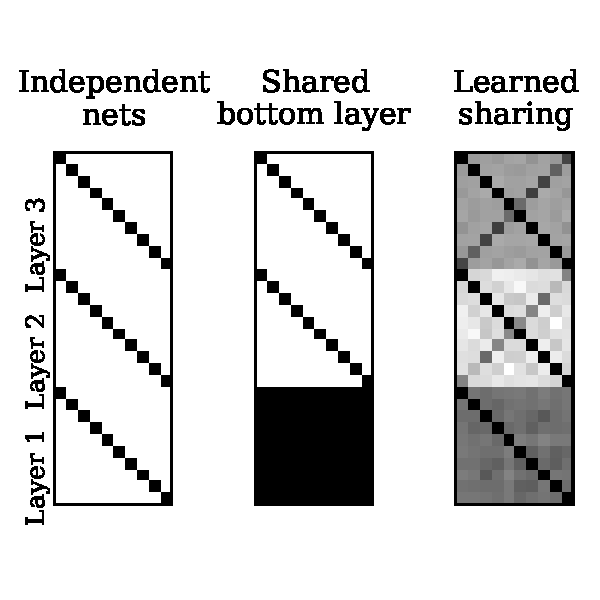
\includegraphics[width=\columnwidth]{../experiments/Feb_4_augmented_omniglot/1/learned_corr.pdf}
%% \begin{tabular}{ccc}
%% Independent & Learned & Full \\
%% \hspace{-1em}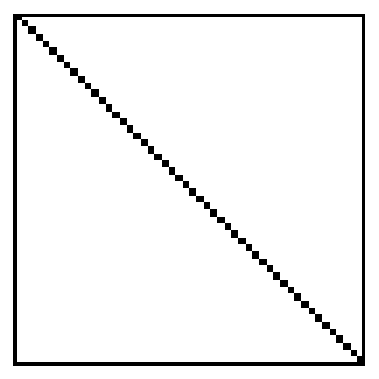
\includegraphics[width=0.31 \columnwidth]{../experiments/Feb_1_learning_alphabet_corr/5/covar_eye.pdf} &
%% \hspace{-1em}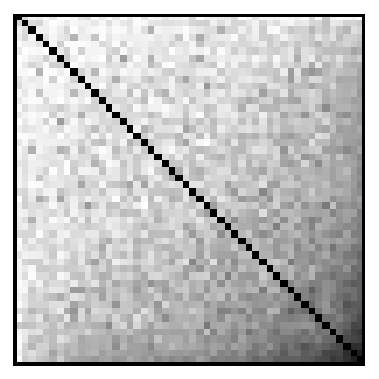
\includegraphics[width=0.31 \columnwidth]{../experiments/Feb_1_learning_alphabet_corr/5/covar_learned_toplayer.pdf} &
%% \hspace{-1em}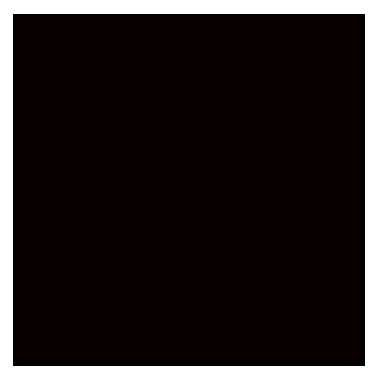
\includegraphics[width=0.31 \columnwidth]{../experiments/Feb_1_learning_alphabet_corr/5/covar_full.pdf}
%% \end{tabular}
\caption{Learned covariances between neural nets trained on different alphabets.}
\label{fig:omniglot}
\end{center}
\end{figure} 



\section{Limitations}

\subsection{When are gradients meaningful?}

\paragraph{Discrete parameters}
Of course gradients are not necessarily useful for optimizing discrete hyperparameters such as the number of layers, or hyperparameters that affect discrete changes such as dropout regularization parameters.
Some of these difficulties could be addressed by 

\subsubsection{Overfitting}

How many hyperparameters can we fruitfully optimize?
The main limitation seems to be overfitting.

[TODO: show the difference between training, validation and test-set error when optimizing]


Gradient-based optimizers can perform poorly when the surface being optimized is locally ``wiggly''.
Small wiggles cause both the direction and size of the gradient to be less correlated with the medium-scale shape of the function.
When do we expect the training loss of a neural network to be wiggly with respect to hyperparameters?

\textbf{The Vanishing Gradient Problem}
Training hyperparameters whose dependence on the final objective depends on many hundreds of iterations by gradient descent raises several issues.
\citet{bengio1994learning} noted that "learning long-term dependencies with gradient descent is difficult."

Exploding-gradient problem~\cite{pascanu2012understanding}

\paragraph{The edge of chaos}
\citet*[Chapter 4]{pearlmutter1996investigation} discusses the chaotic behavior of gradient descent with momentum when training learning neural networks.

One problem with training these networks is that when the learning rate is too high, the gradient becomes uninformative about the medium-term behavior of the function.
Figure \ref{fig:chaos} illustrates this problem.

\cite{pearlmutter2009sleep} argues that biological neural networks tune themselves so as to be at the "edge of chaos".
Empirically, it seems like the best learning rates for training neural networks are just small enough to avoid this chaotic behavior.
Lower learning rates don't reach convergence before training ends.


\begin{figure}[h!]
\vskip 0.2in
\begin{center}
%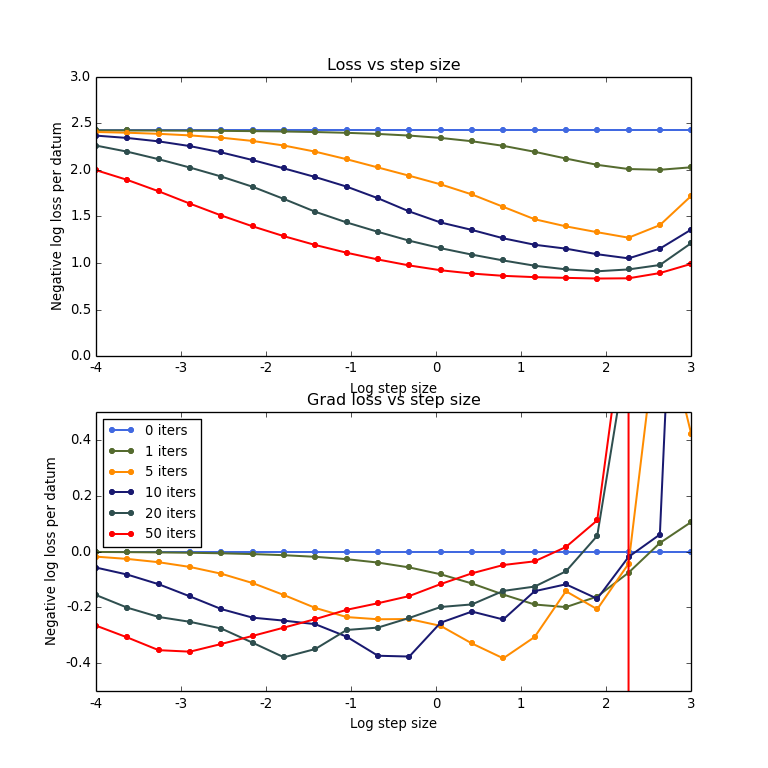
\includegraphics[width=\columnwidth]{../experiments/Jan_14_learning_rate_wiggliness/1/fig.png}
\caption{When the learning rate is too high, the gradient becomes uninformative about the medium-term behavior of the function.
The step sizes which lead to chaotic behavior are only slightly larger than the optimal step sizes.}
\label{fig:chaos}
\end{center}
\vskip -0.2in
\end{figure} 



\section{Related work}

\subsection{Gradient-based tuning of hyperparameters}

\paragraph{Neural networks}
\citet{bengio2000gradient, larsen1998adaptive} identified the benefits of using gradients to optimize the cross-validation loss with respect to neural net hyperparameters, and showed several simple proofs-of-concept.
However, they were only able to compute gradients of hyperparameters that controlled fixed, known functions of the weights, and so could not optimize parameters such as step-sizes or initialization distributions.

\paragraph{Support vector machines}
\citet{chapelle2002choosing} point out that the lack of gradients in the support vector machine (SVM) objective limits the number of kernel parameters, usually to one or two.
They introduced a differentiable bound on the SVM loss in order to be able to compute derivatives with respect to hundreds of hyperparameters, including weighting parameters for each input dimension in the kernel.
However, this bound was not tight. [Need to have another read to figure out limitations of their approach]

\paragraph{Bayesian methods}
For Bayesian methods that have a closed-form marginal likelihood, gradients w.r.t. all continuous hyperparameters are usually available.
for example, this sort of flexibility has been used to construct complex, custom kernels for Gaussian process models~\cite{rasmussen38gaussian}[Chapter 5].
%or to train the parameters of Markov random fields \cite{samuel2012gradient}
Variational inference also allows gradient-based tuning of hyperparameters in Bayesian neural-network models such as deep Gaussian processes~\citep{deepGPVar14}.
However, these methods do not enable the tuning of the parameters which themselves tune the marginal likelihood.

\subsection{Reducing the number of hyperparameters}
Several recent papers have attempted to set training hyper-parameters automatically, or lessen sensitivity to their exact values~\cite{schaul2012no, Adam14, Adasecant14, Hotswap14}.
However, these methods all retain at least a small number of hyperparameters.
In principle, the method we propose here can tune any remaining parameters.
More importantly, having access to hyper-gradients might make the introduction of new, difficult-to-tune hyperparameters worthwhile.

\subsection{Gradients with respect to Markov chain parameters}
\citet{Bridging14} tune the step-size and mass-matrix parameters of Hamiltonian Monte Carlo by chaining gradients from a lower bound on the marginal likelihood through several iterations of leapfrog dynamics.
Because they used only a small number of steps, all intermediate values could be stored naively.
Our reversible-dynamics memory-tape approach could be used to dramatically extend the number of HMC iterations used in this approach.

\section{Extensions and future work}

\paragraph{Long short-term memory}
Several other types of computation performed in machine learning have a similar structure to the reversible dynamics of SGD.
For example, Long Short-Term Memory~\citep{hochreiter1997long} has a similar flavour, as do the computations performed by Neural Turing Machines~\citep{graves2014neural}.
Reversible Learning might allow gradient (not hyper-gradient) computations with respect to very long computations performed by either architecture.

\paragraph{Model-based meta-optimization with gradients}

Current hyper parameter optimization schemes do not usually have access to gradients with respect to these hyperparameters, although Gaussian process-based optimization methods could incorporate this information if it were available~\cite{solak2003derivative}.


\paragraph{Reversible learning using better methods than SGD}

like RMSprop


\section{Conclusion}

In this paper, we derived a computationally efficient procedure for computing gradients through stochastic gradient descent with momentum.
We showed how the approximate reversibility of learning dynamics can be used to drastically reduce the memory requirement for exactly back-propagating gradients through hundreds of training iterations.

We showed how these gradients allow the optimization of validation loss with respect to thousands of hyperparameters, something which was previously infeasible.
This new ability allows the automatic tuning of most details of training neural networks.
We demonstrated the tuning of detailed training schedules, regularization schedules, and neural network architectures.

\section*{Acknowledgments} 

%We would like to thank Christian Steinruecken and Oren Rippel for helpful discussions.

\bibliography{references.bib}
\bibliographystyle{icml2015stylefiles/icml2015}

\end{document} 

